\documentclass{pizzablatt}

\begin{document}

\maketitle{8}{Simon Kapfer, 4. April 2013}

\begin{aufgabe}{Permutationen und lineare Ordnungen}
Vergleiche die beiden Spezies
\begin{itemize}
\item $\textbf{Perm} :\  A \longmapsto \left\{\sigma: A \to A \,|\, \text{$\sigma$ bijektive Abbildung}\right\}$
\item $\textbf{LinO}: \ \;A \longmapsto \left\{\text{Anordnungen der Elemente von }A\ \text{in einer Reihe}\right\}$
\end{itemize}
der Permutationen und der linearen Ordnungen. Begründe, warum gilt:
\begin{align*}
\textbf{Perm}\ &=\ \textbf{E}(\textbf{Cyc}) \\
\textbf{LinO} \ \; &=\ \mathbf{1} + \textbf{X}\cdot \textbf{LinO}  
\end{align*}
Zeige, dass beide Spezies dieselbe erzeugende Funktion besitzen. Sind sie auch
natürlich isomorph?
\end{aufgabe}

\begin{aufgabe}{Oktopoden}
Das nebenstehende Bild zeigt einen Vertreter der \emph{Oktopoden}.
\\
Formuliere eine genaue Definition dieser Spezies.
\marginpar{%
%\hfill\raisebox{0pt}[0pt][0pt]{\vbox{%
    \vspace*{-5em}%
    \hspace*{-10em}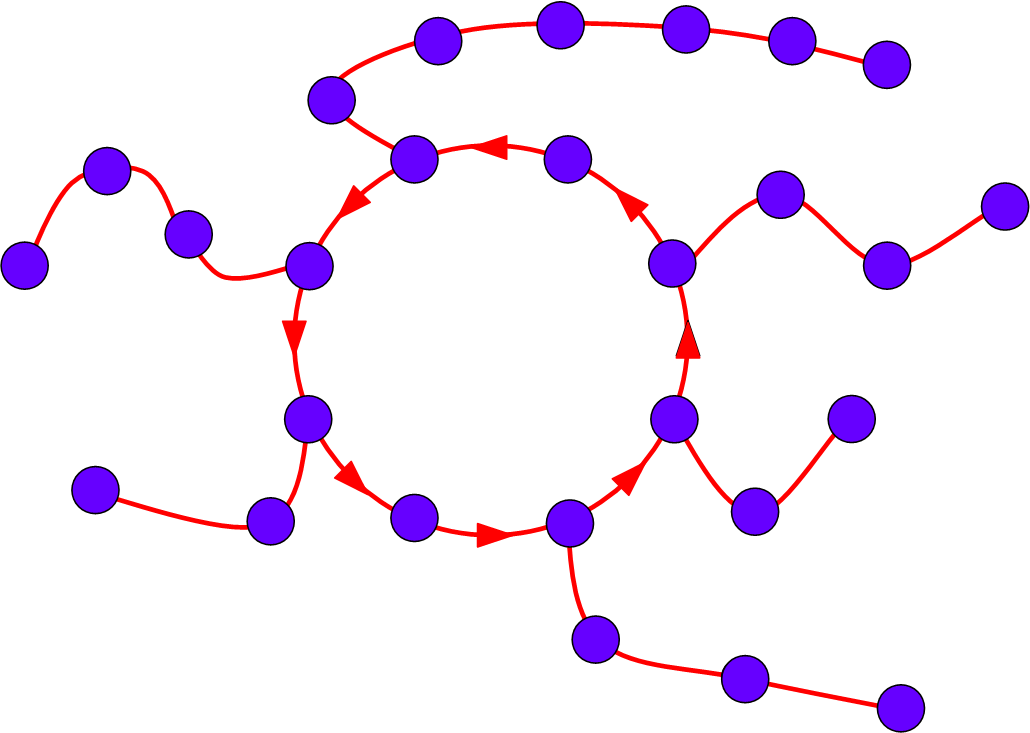
\includegraphics[width=4.5cm]{oktopus.png}}
\end{aufgabe}

\begin{aufgabe}{Botanik}
Auf \url{https://sage.math.uni-augsburg.de/home/pub/0/} finden sich einige
Beispiele zu Bäumen. Passe diese Beispiele für folgende Aufgaben an:
\begin{enumerate}
\item Ein \emph{Rhododendron (Rose Tree)} ist eine Struktur aus Knoten (beginnend
mit einem Wurzelknoten), wobei jedem Knoten ein Wert und eine Liste von
weiteren Knoten (Sprösslingen) zugeordnet ist. Außer dem Wurzelknoten muss
jeder Knoten in genau einer Liste genau einmal vorkommen.

Definiere diese Spezies und berechne die Anzahl der Möglichkeiten, fünf Werte
in Rhododendren zu verpacken. (Antwort: 1680)
\item Ein \emph{Busch} besteht aus einer Anzahl von Blättern und einer Anzahl
von Knoten, verwurzelt an einem Wurzelknoten. Jeder Knoten verzweigt in eine
Menge von~2,~3 oder~4 Sprösslingen. Ein Sprössling kann entweder ein Blatt oder
ein weiterer Knoten sein.

Bastele aus dieser Information eine Spezies und
berechne die Anzahl aller Büsche mit fünf Blättern,
\begin{itemize}
\item falls die Blätter unterscheidbar sind. (Antwort: 235)
\item falls die Blätter nicht unterscheidbar sind. (Antwort: 11)
\end{itemize}
\end{enumerate}
\end{aufgabe}

\begin{tabbing}
  \textbf{Mehr:} \= \kill
  \textbf{Mehr:} \>
  François Bergeron, Gilbert Labelle, Pierre Leroux. \\
  \> \emph{Introduction to the Theory of Species of Structures,} 2008.\\
  \> \small
  \url{http://bergeron.math.uqam.ca/Site/bergeron_uqam_files/livre_combinatoire_2.pdf}
\end{tabbing}

\end{document}
